\documentclass{article}
\usepackage[margin=3cm]{geometry}
%\setlength{\parindent}{0pt}
\usepackage{amssymb}
\usepackage{amsmath}
\usepackage{amsthm}
\usepackage{sectsty}
\usepackage{graphicx}
\usepackage[square,numbers]{natbib}
\usepackage[utf8]{inputenc}
\usepackage[english]{babel}
\usepackage{caption}
\usepackage{subcaption}
\usepackage[hidelinks]{hyperref}
\usepackage[table]{xcolor}

\bibliographystyle{abbrvnat}
%\subsectionfont{\normalfont\itshape}

%\theoremstyle{definition}
\newtheorem{definition}{Definition}[section]
\newtheorem{theorem}{Theorem}[section]

\DeclareMathOperator{\Var}{Var}
\DeclareMathOperator{\VaR}{VaR_\alpha}

\title{Application of Generative Models for \\Risk Measurement in Commodity Trading}
\date{June 20, 2020}

\author{
    \small Vitaliy Pozdnyakov \\
    \small Faculty of Computer Science \\
    \small  \textit{National Research University Higher School of Economics} \\
    \small Moscow, Russia\\
    }

\begin{document}

\maketitle

\abstract{Generative models in machine learning allow to estimate a joint probability distribution over observed data. Using such models, it is possible to generate new observations by Monte Carlo simulations and analyze a resulting empirical distribution numericalally. In this work I will consider three generative models: Geometric Brownian Motion, Copulas and Generative Adversarial Network. The goal of this work is to compare the quality of these models in the task of risk measurement in commodity trading.}

\tableofcontents

\newpage

\section{Introduction}
A complete and exhaustive description of generative and discriminative approaches in machine learning was formulated in \cite{jebara}. The main difference between the approaches is represented by a degree of statistical modeling. The generative approach describes models of joint probability distribution over all considered random variables. Having a fairly accurate model of a distribution, it is possible to solve classification and regression problems using numerical methods for calculating conditional probabilities and moments. For example, for $n$ random variables $(X_1, \dots, X_n)$ and the known joint distribution we can calculate a probability that the observation $\{X_i = x_i\}_{\forall i \neq j}^{n}$ belongs to the class $X_j = x_j$ (in a descrete case): 
\begin{align*}
    P(X_j = x_j| \{X_i = x_i\}_{\forall i \neq j}^n) =
\frac{P(X_j = x_j, \{X_i = x_i\}_{\forall i \neq j}^n)}{\sum_{k} P(X_j = x_k, \{X_i = x_i\}_{\forall i \neq j}^n)}
\end{align*}
In practice, however, we often cannot find the probability explicitly, but we can obtain approximate solution by a Monte Carlo simulation — to randomly generate a set of observations from the generative model $X_j| \{X_i = x_i\}_{\forall i \neq j}$ and then calculate a proportion of observations for which $X_j = x_j$. Popular generative models include Bayesian networks, autoregressive models, variational autoencoders, generative adversarial networks.

The discriminative approach describes models for directly calculating a result of classification or regression from input observation. These models do not analyze a joint distribution over all variables, but focus only on optimizing a predictor to obtain the most accurate estimate of the target variable. Such models are usually simpler and faster, because they do not apply any intermediate steps to get the result. Popular discriminative models include linear regression, logistic regression, support vector machines, neural networks, decision trees, gradient boosting.

Despite the fact that generative models provide a more complete picture of the behavior of random variables, such models can be more computationally expensive and non-robust \cite{jebara}. Also, as was shown in \cite{Ng2002}, generative models have a higher asymptotic error, but on the other hand, with growth of observations, they approach an asymptotic error much faster than discriminative models, which allows to use generative models more effectively on relatively small datasets. Thereby the choice of approach depends on the specific problem. 

In this work I will consider the problem of risk measurement in commodity trading. Traditionally, commodity trading firms (CTFs) use the Value-at-Risk (VaR) metric to measure their risk \cite{Pirrong}. VaR defines a bound of the amount of money that would be lost on a given time horizon with a given confidence level. For example, if a time horizon is 1 day, a confidence level is 95\% and VaR is \$10 millions, this means that in 95\% of trading days a company expects to lose no more than \$10 millions, and vice versa, in the remaining 5\% of trading days a company expects to lose more than \$10 millions. More formally, VaR was defined in \cite{Artzner1999}.
\begin{definition}[Value-at-Risk]
    Value-at-Risk of a given asset or portfolio profit, at the confidence interval $\alpha$, is given by
$$\VaR(X) := -\inf\{ x \in \mathbb R | F_X(x) > \alpha\}$$
where $F_X$ is cumulative distribution function of $X$. 
\end{definition}

According to this definition, a confidence level 95\% coincides with $\alpha = 0.05$.  In addition, CTFs often uses the Conditional VaR metric (CVaR), which determines the average value of losses if VaR is exceeded. Generative models are widely used to calculate these metrics, since they allow to conveniently evaluate and visualize VaR and CVaR on any quantiles. In this work I will consider VaR and CVaR with respect to three generative models: Geometric Brownian Motion (GBM), Copula, Generative Adversarial Network (GAN).

\section{Related works}
\label{section:related}
\textbf{Geometric Brownian Motion (GBM)}. In literature, GBM is often used to model stock prices, commodity prices, changes in demand for products and services, as well as to analyze options \cite{BENNINGA}, \cite{Nembhard}, \cite{Thorsen}. In \cite{Nkemnole}, modifications of GBM using Student's t distribution were considered for modeling various time series, including for modeling gas and crude oil prices. The purpose of the study was to compare student's t GBM with normal GBM. Experimental comparison of generated and real data showed that Student's t GBM is more highly accurate than the Gaussian GBM as proved by the lower than 10\% MAPE value. The paper \cite{Croghan2017EstimationOG} is also dedicated to use of GBM for modeling crude oil and gas prices. Three methods for evaluating GBM parameters were considered: based on a ratios of the difference between observations, based on the maximum likelihood estimation, and also based on log ratios. Experimental results have shown that all three methods have approximately the same accuracy, but log ratios do not have a normal distribution, so potentially this method may not give an accurate estimate. \cite{Lidn2018StockPP} used 10 years of observed Apple stock prices and S\&P500 index values, compared GBM and ARMA+GARCH models to predict prices. Experimental results showed that both models have approximately the same accuracy, which coincided with the results in \cite{Reddy}.

\textbf{Copulas}. Copulas are used for modeling dependencies between variables in the field of risk management. In \cite{Stefano2005}, it was shown that copulae are more flexible and precise than the Variance-Covariance Method. The exception is Gaussian copula, which showed a fairly weak result in \cite{Thorsen}. The article \cite{Kole2006} is devoted to use of various copulas for the task of risk measurement with respect to VaR and a possibility of diversification of portfolios of stocks, bonds and real estate. Computational experiments have shown that Gaussian copula underestimates the risk of extreme portfolio losses, while Gumbel copula overestimates it. As a result, it was concluded that Student's t copula is more preferable than Gaussian copula and Gumbel copula. However, as shown in \cite{Patki2016}, Gaussian copula can be successfully used as a universal tabular data generation tool for various machine learning tasks.

\textbf{Generative Adversarial Network (GAN)}. GAN model was proposed in \cite{goodfellow2014generative} and is usually used to generate images \cite{radford2015unsupervised} or even to generate images from another image or text. The Tabular GAN (TGAN) model was proposed for generating tabular data in \cite{xu2018synthesizing}. A matrix of normalized mutual information values was calculated for each dataset based on real and synthetic data, and RSME and MAE metrics were compared for various generative models. As a result of experiments, it was shown that TGAN outperformes the quality of the Gaussian copula and Bayesian networks.

\section{Generative Models}
\label{section:models}

\subsection{Geometric Brownian Motion}
\label{section:gdm}

Stochastic differential equations model processes that are subject to random fluctuations, but have long-term trends. Stock prices or commodity prices on the market can be considered as stochastic processes, which can be expressed by stochastic differential equations of the form (according to\cite{Lidn2018StockPP})

\begin{equation*}
\begin{cases}
dX(t) = \mu X(t) dt + \sigma X(t) d W(t) \\
X(0) = x_0
\end{cases}
\end{equation*}
where $W(t)$ is a Wiener process (continuous-time Gaussian process with independent increments), $\mu$ and $\sigma > 0$ represent drift and volatility constants, $t$ is a time moment. There is a well known \cite{Lidn2018StockPP} explicit solution
\begin{equation*}
X(t) = X_0 \exp\left[ \left(\mu - \frac{\sigma^2}{2} \right) t + \sigma W(t) \right].
\end{equation*}
Parameters $\mu$ and $\sigma$ can be estimated by the Method 1 from the paper \cite{Croghan2017EstimationOG} as follows
\begin{equation*}
\hat{\mu}=\sum_{t=1}^{n} \frac{X(t)-X(t-1)}{X(t-1)},
\end{equation*}
\begin{equation*}
\hat{\sigma}=\sqrt{\frac{1}{n-1} \sum_{t=1}^{n}\left(\frac{X(t)-X(t-1)}{X(t-1)}-\hat{\mu}\right)^{2}}
\end{equation*}
where $n$ is the number of observations. 

The multidimensional extension of GBM was described in \cite{sabino2007monte} as the vector $$(X_1(t), X_2(t), \dots, X_m(t))^T$$ with a correlated Wiener processes of the form
\begin{equation*}
\begin{bmatrix}
    W_i(0)\\
    W_i(1)\\
    \dots \\
    W_i(n)
\end{bmatrix} = C_R \begin{bmatrix}
    \mathcal{N}_{0, 1}\\
    \mathcal{N}_{0, 1}\\
    \dots\\
    \mathcal{N}_{0, 1}
\end{bmatrix}
\end{equation*}
where $C_R$ is the Cholesky decomposition of the autocorrelation matrix $\mathbf P$. The estimation of the autocorrelation matrix can be given as the empirical autocorrelation matrix $\hat {\mathbf P}$. In Figure \ref{fig:gbm1} shows an example of three runs by two GBMs with high correlation that start from the same position.

\begin{figure}[h]
    \centering
    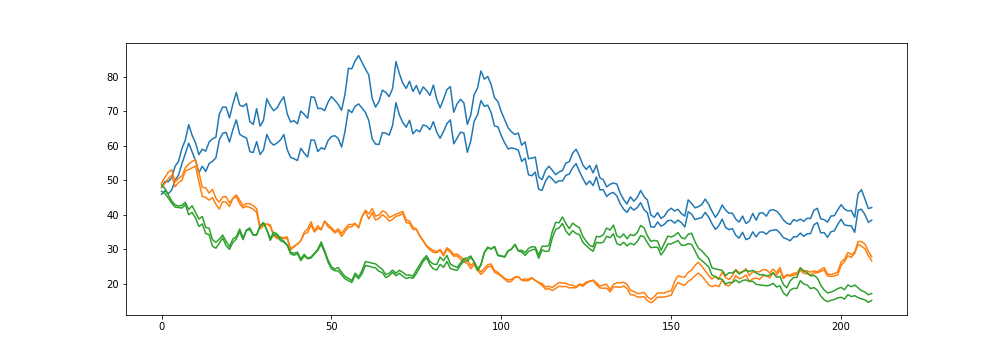
\includegraphics[width=0.8\textwidth]{pics/gbm.png}
    \caption{Example of three runs by two high-correlated GBMs}
    \label{fig:gbm1}
\end{figure}

\subsection{Copulas}
\label{section:copulas}

A copula is a function that allows us to split a multidimensional distribution into separate components: marginal distributions and dependency sctructure between random variables. This way of representing a multidimensional distribution is very useful for several reasons. First, we can apply methods of statistical analysis separately for each of the components and managed independently from each other, it provides flexibility in modelling multivariate distributions. Second, this method provides a convenient tool for independent generation of observations, which is widely used in risk measurement.

\begin{definition}[Copula]
    For the given d-dimensional random vector $(X_1, X_2, \dots, X_d)$ copula is defined as a cumulative distribution function (CDF) $C: [0, 1]^d \to [0, 1]$ of the form
    $$C(u_1, u_2, \dots, u_d) = P(X_1 \leq F_1^{-1}(u_1), X_2 \leq F_2^{-1}(u_2), \dots, X_d \leq F_d^{-1}(u_d))$$
    where $F^{-1}_i$ is a reverse CDF of $X_i$ RV and $u_i$ is a i-th uniform value.
\end{definition}

A copula is a universal tool for modeling any distributions with marginals, which is confirmed by Sklar's theorem \cite{lo2018simple}.
\begin{theorem}[Sklar’s Theorem 1959]
    For any CDF $F$ on $\mathbb R^d, d \geq 1$ there exists a copula $C$ on $\mathbb R^d$ such that
    $$\forall x\in \mathbb R^d, F(x) = C(F_1(x), \dots, F_d(x)).$$
\end{theorem}

This theorem is very important in Statistics since it allows to model dependence between components of a random vector independently of the marginals. One of the most popular examples of a copula for risk measurement is the $t$ copula. The $d$-dimensional $t$-copula is defined as
$$
C_{\nu, P}^{t}(\mathbf{u}):=\mathbf{t}_{\nu, \mathbf{P}}\left(t_{\nu}^{-1}\left(u_{1}\right), \ldots, t_{\nu}^{-1}\left(u_{d}\right)\right)
$$
where $\mathbf{P}$ is a correlation matrix, $\mathbf{t}_{\nu, \mathbf{P}}$ is the joint $\mathrm{CDF}$ of $\mathbf{X} \sim \mathbf{t}_{d}(\nu, \mathbf{0}, \mathbf{P})$ and $t_{\nu}$ is the standard univariate CDF of a $t$-distribution with $\nu$ degrees of freedom. Generating observations from the $t$ copula is performed as follows:

\begin{enumerate}
    \item Generate $n$ observations from a $d$-dimensional $t$-distribution using fitted correlation matrix $P$ and degrees of freedom $\nu$.
    $$(\mathbf{t}_1, \mathbf{t}_2, \dots, \mathbf{t}_n), \mathbf{t}_i \sim t_d(\nu, \mathbf{0}, \mathbf{P} ).$$
    An example is in Figure \ref{fig:copula1}.
    \item Use CDF for each marginal component of the observation to get $n$ uniform observations. Let $\mathbf{t} = [t_{1}, t_{2}, \dots, t_{d}]$, then each separate observation takes the form
    $$(u_1, u_2, \dots, u_d) = \left[t_{\nu}(t_{1}), t_{\nu}(t_{2}), \dots, t_{\nu}(t_{d})\right]$$
    where $t_{\nu}$ is the standard univariate CDF of a $t$-distribution with $\nu$ degrees of freedom. An example is in Figure \ref{fig:copula2}.
    \item Finally, apply the reverse CDFs of marginal distributions $F_1, F_2, \dots, F_d$ to get the final modeled distribution. Each observation takes the form
    $$(x_1, x_2, \dots, x_d) = \left[ F_1^{-1}(u_1), F_2^{-1}(u_2), \dots, F_d^{-1}(u_d) \right].$$
    For example, the marginal distributions $F_1, F_2, \dots, F_d$ can be set using the Kernel Density Estimator (KDE). An example of the obtained observations is in Figure \ref{fig:copula3}.
\end{enumerate}

\begin{figure}[!ht]
    \begin{minipage}{.33\linewidth}
        \centering
        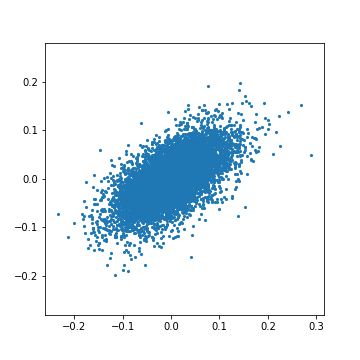
\includegraphics[width=\textwidth]{pics/copula1.png}
        \subcaption{Multivariate $t$-distribution}
        \label{fig:copula1}
    \end{minipage}%
    \begin{minipage}{.33\linewidth}
        \centering
        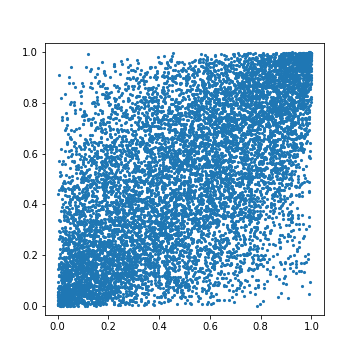
\includegraphics[width=\textwidth]{pics/copula2.png}
        \subcaption{Uniform transformation}
        \label{fig:copula2}
    \end{minipage}
    \begin{minipage}{.33\linewidth}
        \centering
        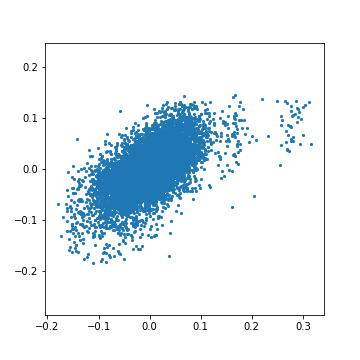
\includegraphics[width=\textwidth]{pics/copula3.png}
        \subcaption{KDE marginals}
        \label{fig:copula3}
    \end{minipage}
    \caption{Example of $t$ copula generation step-by-step}
    \label{fig:mem}
\end{figure}

\subsection{Generative Adversarial Networks}
\label{section:gan}
The Generative Adversarial Networks (GAN) consists of two parts: the generator $G$ and the discriminator $D$. The task of the discriminator $D$ is to distinguish generated data from real data, while the task of the generator $G$ is to "trick" the discriminator by generating more and more accurate data. GANs differ in architecture depending on which models are selected for the generator and discriminator. In my work I use architecture proposed in \cite{xu2018synthesizing} and provided in an open source Python package \cite{tgan}. The generator use long-short-term memory (LSTM) network, and the discriminator use Multi-Layer Perceptron (MLP). Here I briefly describe architecture of this GAN.

\textbf{Generator $G$}. The size of an output and hidden state of the LSTM is denoted by $n_h$. A random variable $z$ is fed to the LSTM input at each time $t$, as well as a hidden vector $f_{t-1}$ or an embedding vector $f'_{t-1}$, depending on the type of previous output. The weighted context vector $a_{t-1}$ is also fed to input. The random variable $z$ has dimension $n_z$ and each dimension is generated from the distribution $N(0, 1)$. The context vector $a_t$ weighted by all previous outputs of the LSTM has the dimension $n_h$. The $a_t$ vector is calculated as
$$a_{t}=\sum_{k=1}^{t} \frac{\exp (\alpha_{t, k})}{\sum_{j} \exp (\alpha_{t, j})} h_{k}.$$
$A_0$ is set to 0. Exit from LSTM is denoted by $h_t$. Using the training parameter $W_h$, there is a getting projection of the vector $h_t$ of the form $f_t = \text{tanh}(W_hh_t)$ and the size $n_f$. Next, the hidden vector is converted to the output value as follows: $v_i = \text{tanh}(W_hf_t)$. The hidden vector for $t+1$ is $f_t$.

\textbf{Discriminator $D$}. A $l$-layer fully connected neural network is used for the discriminator. The network input receives the concatenation result $v_{1:n_c}, u_{1:n_c}$ and $d_{1:n_d}$. Internal layers are calculated as follows
$$f_{1}^{(D)}=\operatorname{LeakyReLU}\left(\operatorname{BN}\left(W_{1}^{(D)}\left(v_{1: n_{c}} \oplus u_{1: n_{c}} \oplus \mathbf{d}_{1: n_{d}}\right)\right)\right),$$
$$f_{i}^{(D)}=\operatorname{LeakyReLU}\left(\operatorname{BN}\left(W_{i}^{(D)}\left(f_{i-1}^{(D)} \oplus \operatorname{diversity}\left(f_{i-1}^{(D)}\right)\right)\right)\right), i=2: l$$
where $\oplus$ is the concatenation operation. diversity $(\cdot)$ is the mini-batch discrimination vector. Each dimension in the diversity vector is defined by the distance of one sample to all the others in the mini-batch. BN$(\cdot)$ is batch normalization, and LeakyReLU$(\cdot)$ is a leaky reflect linear activation function. To calculate the discriminator output, there is used the scalar $W^{(D)}(f^{(D)} \oplus diversity(f^{(D)}))$.

\textbf{Loss Function}. Since the model is differentiable, the Adam optimizer is used here. To optimize the generator, use

$$
\mathcal{L}_{G}=-\mathbb{E}_{z \sim \mathcal{N}(0,1)} \log D(G(z))+\sum_{i=1}^{n_{c}} \operatorname{KL}\left(u_{i}^{\prime}, u_{i}\right)+\sum_{i=1}^{n_{d}} \operatorname{KL}\left(\mathbf{d}_{i}^{\prime}, \mathbf{d}_{i}\right)
$$
where $u_{i}^{\prime}$ and $\mathbf{d}_{i}^{\prime}$ are generated data while $u_{i}$ and $\mathbf{d}_{i}$ are real data, KL$(\cdot, \cdot)$ is the Kullback–Leibler divergence of discrete variables and the cluster vector of continuous variables. There is an optimizing the discriminator using conventional cross-entropy loss
$$
\mathcal{L}_{D}=-\mathbb{E}_{v_{1: n_{c}}, u_{1: n_{c}}, \mathbf{d}_{1: n_{d}} \sim \mathbb{P}(\mathbf{T})} \log D\left(v_{1: n_{c}}, u_{1: n_{c}}, \mathbf{d}_{1: n_{d}}\right)+\mathbb{E}_{z \sim \mathcal{N}(0,1)} \log D(G(z)).
$$

\section{Commodity trading}
\label{section:case}
\subsection{Transformation categories}

Agricultural, energy and industrial commodities undergo transformations before they can be sold to a final buyer, consumed, or used. In the economics of commodity trading review \cite{Pirrong} identifies three types of transformations:
\begin{itemize}
    \item in space (logistics)
    \item in time (storage)
    \item in form (processing)
\end{itemize}

Usually regions where commodities are produced (for example, fertile land or mineral deposits) are located far enough away from regions where they are desired to be consumed. So, space transformation involves transporting commodities from region where these commodities are produced to regions where they are consumed.

Time transformation eliminates a discrepancy between a period of commodity consumption and a period of production. This is especially evident in agricultural commodities, which have a pronounced seasonality -- a crop is harvested once a year, but consumption persists all year round. In addition, some commodities are highly susceptible to fluctuations that are random in nature, such as weather conditions, macroeconomic events, and financial crises. In these cases, CTFs can also use a time transformation to wait for a better moment to sell a commodity.

Transformation by form includes processing, cleaning, and recycling of commodity. These procedures may be intended for preparing a commodity for sale to the end user or for an intermediate stage of transformation. For example, crude oil must be transformed into gasoline, diesel, or other fuel in order to be used by the end user.

\subsection{Challenges in commodity trading}

Companies that perform the transformations are called Commodity Trading Firms (CTFs). The main objectives of CTFs are noticed in the economics of commodity trading review \cite{Pirrong}.

First, they are engaged in a search of an "arbitrage" -- a situation when benefits of a commodity transformation exceed a price of a transformation itself. Thus, commodity traders perform simultaneous purchase and selling of commodities different forms. It follows that firms are primarily concerned with a difference between prices, not with absolute values of prices. A profit from a trader's work depends on a price difference between untransformed and transformed commodities much more than on an absolute level of these prices.

Second, they are searching for the most optimal transformation for a commodity. This is a dynamic process that depends on multiple supply and demand shocks. For example, a good harvest in one region may entail storing this commodity, or transporting it to another region. A process of performing transformations is highly dependent on technological equipment and on availability of infrastructure. For example, availability of air, water, and land transport determines possible types of transformations.

\subsection{Risks in commodity trading}

There are different categories of CTFs risks. For example, Flat price risk indicates a risk of a drop in a commodity price before selling. The Basis Risk arises in a case of commodity hedging with derivatives, prices of which can also change significantly. Spread risk is a calendar (or time) spread trade in which the same commodity is bought and sold simultaneously, for different delivery dates. Many commodity hedges involve a mismatch in timing that gives rise to spread risk.

For risk measurement, many CTFs use the Monte-Carlo simulations method to predict results of various scenarios. Generally, a risk is based on the VaR metric with a confidence level of 95\% and a time horizon of one day \cite{Pirrong}. In addition, the CVaR metric is evaluated for the same parameters.

\section{Dataset description}
\label{section:dataset}
For this work I use the Rogers International Commodity Index, which is a set of indices with a wide range of commodities consumed in the global economy. Weighted values of the index is estimated using futures contracts for exchange-traded physical goods consisting of 38 commodities. All commodities are divided into three indexes: Energy, Metals and Agriculture. I use the energy \cite{RICI} index, which consists of 6 energy commodities:

\begin{itemize}
    \item Crude Oil -- 37.50\% (called as \texttt{crude} in the figures)
    \item Brent -- 32.50\% (\texttt{brent})
    \item Natural Gas -- 15.00\% (\texttt{natural})
    \item RBOB Gasoline -- 7.50\% (\texttt{gasoline})
    \item Heating Oil -- 4.50\% (\texttt{heating})
    \item Gas Oil 3.00\% (\texttt{gas})
\end{itemize}

Commodity prices were downloaded from the site \url{https://investing.com/} for the period 01.01.2008 - 01.06.2020 in one-day increments, a total of 3476 observations. To compare the commoditity between them I convert the absolute prices to returns values of the form
$$r_t = \frac{x_t - x_{t-1}}{x_{t-1}}.$$
Obtained time series for Aug-Oct 2008 is shown in Figure \ref{fig:returns}. The resulting correlation matrix is shown in Figure \ref{fig:heatmap}. As we can see, there is the highest correlation between Brent and Heating Oil commodities (0.87), Natural Gas and Gas Oil have the lowest correlation (0.12), there are no negatively correlated commodities.

\begin{figure}[h]
    \centering
    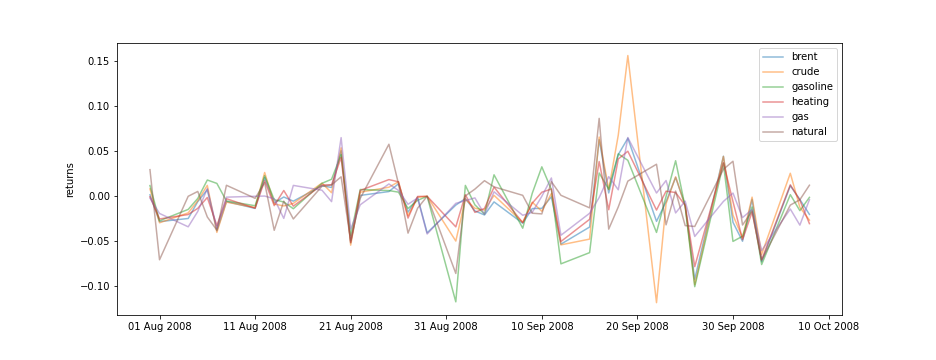
\includegraphics[width=0.8\textwidth]{pics/returns.png}
    \caption{Time series by returns of commodities}
    \label{fig:returns}
\end{figure}

\begin{figure}[h]
    \centering
    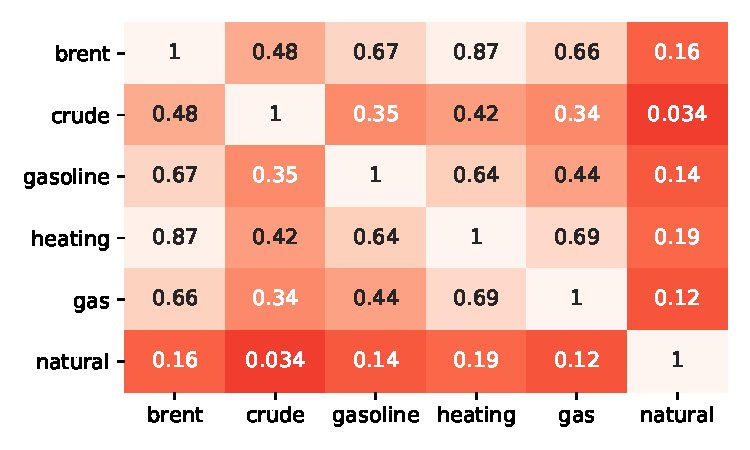
\includegraphics[width=0.5\textwidth]{pics/heatmap.pdf}
    \caption{Correlation matrix of commodities by returns}
    \label{fig:heatmap}
\end{figure}

\section{Computational results}
\label{section:results}
The following models participated in testing:
\begin{itemize}
    \item GBM
    \item $t$ copula, $t$ marginals
    \item $t$ copula, Gaussian KDE marginals
    \item GAN
\end{itemize}

To test the quality of models, I take the first 70\% of observations: from 01.01.2008 to 23.01.2017. These observations I use to train the models. I fit GBM according to as specified in Section \ref{section:gdm}. To generate observations from $t$ copula, two parameters are required: the correlation matrix and the number of degrees of freedom. I evaluate the correlation matrix using an empirical correlation matrix. The number of degrees of freedom I estimate as the average value of degrees of freedom for all estimates of degrees of freedom of marginal distributions. To evaluate the parameters of $t$ marginals, I use the MLE method. For KDE marginals, the Kernel Density Estimation algorithm itself is used, and Gaussian distributions were used as kernel densities.

I select the following parameters for GAN training (either empirically selected or using the default values set by the developers):
\begin{itemize}
    \item Number of epochs to use during training: 5
    \item Number of steps to run on each epoch: 10000
    \item Size of the batch to feed the model at each step: 200
    \item Number of dimensions in the noise input for the generator: 100
    \item Upper bound to the gaussian noise added to categorical columns: 0.2
    \item L2 reguralization coefficient when computing losses: 0.00001
    \item Learning rate for the optimizer: 0.001
    \item Number of units in RNN cell in the generator: 400
    \item Number of units in fully connected layer in the generator: 100
    \item Number of layers in the discriminator: 2
    \item Number of units per layer in the discriminator: 200
\end{itemize}

After training, I generate 10,000 observations from the models and compared them with observations from the test set (from 24.01.2017 to 01.06.2020). Figure \ref{fig:gens} shows an example of real and generated observations in the context of RBOB Gasoline and Natural Gas commodities. We can notice that the GBM model has shorter tails, this can be explained by the Gaussian distribution that underlies this model. The $t$ copula, $t$ marginals model has heavier tails that are distributed more evenly across the entire plane. The $t$ copula, Gaussian KDE marginals model also has wider tails, but the distribution is shifted to the right side of the plane. GAN has generated observations on a complex dependency structure, here we can see stable clusters of points in certain areas of the plane, so visually, it seems that the GAN model is prone to overfitting. Since I have generated 10000 observations from each model, I sort a sequence of these observations day-by-day to obtain a set of paths of price changes. The test set consists of about 1000 days, so I construct 10 paths by each model. The generated paths of Brent price is also depicted in Figure \ref{fig:paths}. The $t$ copula, $t$ marginals model has generated a few significant outliers, while other models seems more stable.

\begin{figure}[!ht]
    \begin{center}
        \begin{minipage}{.33\linewidth}
            \centering
            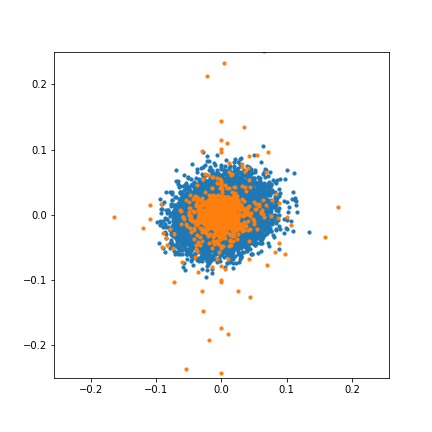
\includegraphics[width=\textwidth]{pics/gen_gbm.png}
            \subcaption{GBM}
            \label{fig:gen_gbm}
        \end{minipage}%
        \begin{minipage}{.33\linewidth}
            \centering
            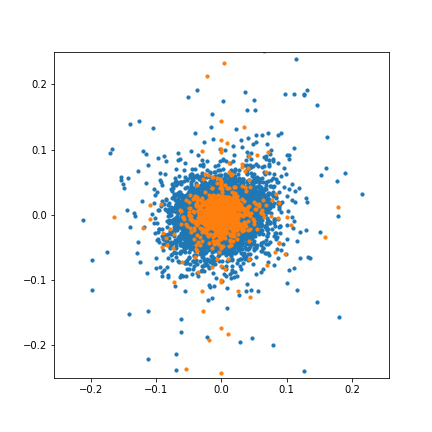
\includegraphics[width=\textwidth]{pics/gen_t_copula.png}
            \subcaption{$t$ copula, $t$ marginals}
            \label{fig:gen_t_copula}
        \end{minipage}
        \begin{minipage}{.33\linewidth}
            \centering
            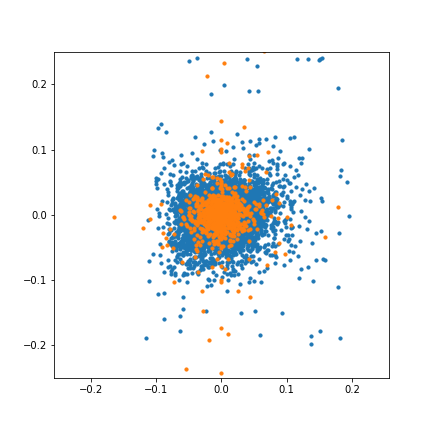
\includegraphics[width=\textwidth]{pics/gen_t_copulaKDE.png}
            \subcaption{$t$ copula, KDE marginals}
            \label{fig:gen_t_copulaKDE}
        \end{minipage}%
        \begin{minipage}{.33\linewidth}
            \centering
            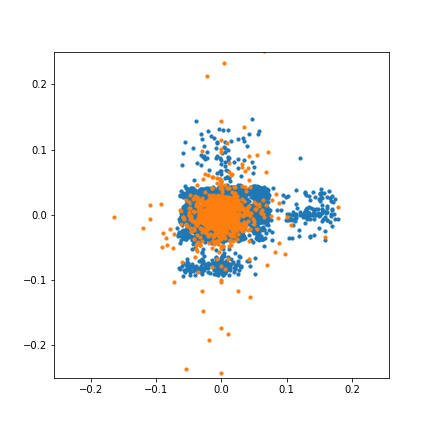
\includegraphics[width=\textwidth]{pics/gen_tgan.png}
            \subcaption{GAN}
            \label{fig:gen_tgan}
        \end{minipage}
        \caption{Generated (blue) and real (orange) observations, \\Natural Gas vs RBOB Gasoline}
        \label{fig:gens}
    \end{center}
\end{figure}

\begin{figure}[!ht]
    \begin{center}
        \begin{minipage}{.5\linewidth}
            \centering
            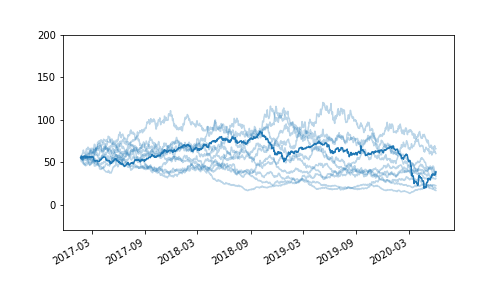
\includegraphics[width=\textwidth]{pics/path_gbm.png}
            \subcaption{GBM}
            \label{fig:gbm_path}
        \end{minipage}%
        \begin{minipage}{.5\linewidth}
            \centering
            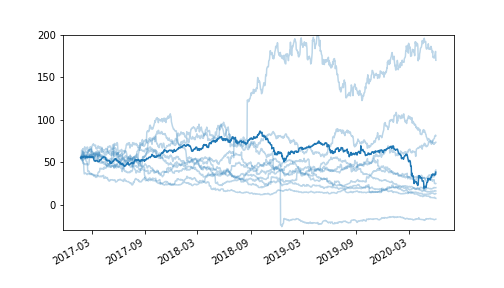
\includegraphics[width=\textwidth]{pics/path_t_copula.png}
            \subcaption{$t$ copula, $t$ marginals}
            \label{fig:t_copula_path}
        \end{minipage}
        \begin{minipage}{.5\linewidth}
            \centering
            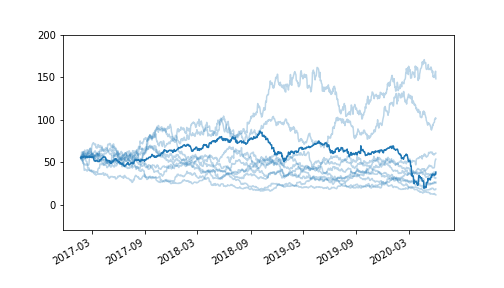
\includegraphics[width=\textwidth]{pics/path_t_copulaKDE.png}
            \subcaption{$t$ copula, KDE marginals}
            \label{fig:t_copulaKDE_path}
        \end{minipage}%
        \begin{minipage}{.5\linewidth}
            \centering
            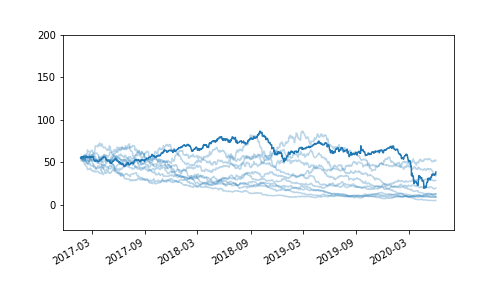
\includegraphics[width=\textwidth]{pics/path_tgan.png}
            \subcaption{GAN}
            \label{fig:tgan_path}
        \end{minipage}
        \caption{Generated and real (bright) paths of the Brent price}
        \label{fig:paths}
    \end{center}
\end{figure}

I apply Kolmogorov-Smirnov test (KS) and Kullback–Leibler divergence (KL) to compare generation quality. To calculate a single value for all commodities for Kolmogorov-Smirnov test, I use the average value for all commodities, for Kullback-Leibler divergence I use the sum for all commodities. The test results are shown in Table \ref{tab:quality}.

\begin{table}[h]
    \begin{center}
    \begin{tabular}{ |c|c|c|c| } 
    \hline
    Model & KS statistic & KL \\ 
    \hline
    GBM & 0.1282 & 1.064 \\ 
    $t$ copula, $t$ marginals & 0.1031 & \textbf{0.111} \\ 
    $t$ copula, KDE marginals & \textbf{0.1028} & 0.338 \\ 
    GAN & 0.1491 & 0.873 \\ 
    \hline
    \end{tabular}
    \end{center}
    \caption{Values of Kolmogorov-Smirnov test (KS) \\and Kullback–Leibler divergence (KL)}
    \label{tab:quality}
\end{table}

To calculate the VaR, I use a commodity portfolio with a total amount \$100000, where each commodity is weighted with respect to Rogers International Commodity Index. I use prices at the end of the train set (23.01.2017). I calculate the one day profit as
$$\text{profit}_t = \sum_{i=1}^6 r_{t,i} \times w_i$$
with $i \in \{1, 2, 3, 4, 5 , 6\}$ commodities, returns values $r_{t, i}$ and weights by index $w_i$. Calculated profit values is represented by smooth and normalized histograms in Figure \ref{fig:profit}. We see that $t$ copula has heavier tails than GAN and GBM, and is noticeably closer to real values.

I calculate VaR and CVaR with one day time horizon and 95\% confidence level using obtained distributions. The resulting values by models are represented in Table \ref{tab:var} as well as the real VaR and CVaR values based on one day profits from the test set of observations.

\begin{figure}[h]
    \centering
    \begin{minipage}{.5\linewidth}
        \centering
        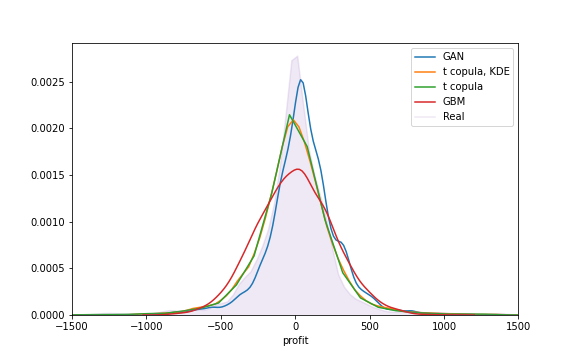
\includegraphics[width=\textwidth]{pics/hists.png}
    \end{minipage}%
    \begin{minipage}{.5\linewidth}
        \centering
        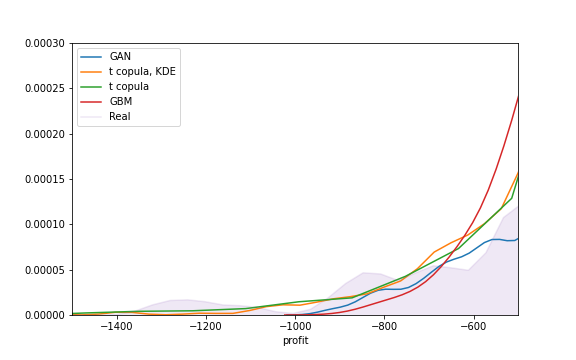
\includegraphics[width=\textwidth]{pics/tails.png}
    \end{minipage}%
    \caption{Profit distribution by Rogers International Commodity Index}
    \label{fig:profit}
\end{figure}

\begin{table}[h]
    \begin{center}
    \begin{tabular}{ |c|c|c|c| } 
    \hline
    Model & VaR & CVaR \\ 
    \hline
    Real value & 374.31 & 682.30 \\ 
    \hline
    GBM & 420.66 & 526.82 \\ 
    $t$ copula, $t$ marginals & \textbf{402.56} & \textbf{638.26} \\ 
    $t$ copula, KDE marginals & 404.33 & 585.49 \\ 
    GAN & 319.36 & 488.77 \\ 
    \hline
    \end{tabular}
    \end{center}
    \caption{VaR and CVaR values}
    \label{tab:var}
\end{table}

\section{Conclusion}
\label{section:conclustion}
In this work, I reviewed quality of three generative models: Geometric Brownian Motion, Copulas (two options: with $t$ marginals and KDE marginals) and Generative Adversarial Network. I used data on daily commodity prices on exchanges in the period 01.01.2008-01.06.2020. As a result of computational experiments, it was shown that the $t$ copula models have the best accuracy relative to Kolmogorov-Smirnov test. Regarding Kullback-Leibler divergence, the best result was also shown by the $t$ copula, $t$ marginals model. Both $t$ copulas models have heavier tails, which is typical for the  distribution of our data.

For the task of risk measurement I have used the VaR and CVaR metrics regarding the portfolio of commodities is compiled by the Rogers International Commodity Index: Energy. The obtained results tell us that the $t$ copula, $t$ marginals model was the most accurate in the risk measurement problem for both metrics. GBM overestimates VaR, while GAN underestimates. The metric CVaR was underestimated by all models, however, the $t$ copula, $t$ marginals turned out to be accurate.

Further research on this topic can be continued in the direction of modification and search for optimal GAN parameters to get rid of overfitting. In addition, it is reasonable to considered novel models that combine copulas and autoencoders models \cite{tagasovska2019copulas}, as well as GBM based on the $t$ distribution \cite{Nkemnole}.

\bibliography{main}

\end{document}
